\chapter{Experimental Setup, Methodology and Calibration}




\section{Experimental Setup: 3D-Printed Mounts}
\label{sec:experimental_setup}

This section describes the physical assembly used for all the measurements of this chapter. To obtain a compact and low-cost measurement system, a set of modular parts was prototyped in CAD and printed in FDM (fused deposition modeling) 3D printing. The parts hold the interferometer, couple it to the optical detectors and let the camera and the photodiode be used at the same time. The designs are shown in \cref{fig:printed_parts_main,fig:printed_parts_detectors}.

\begin{figure}[htbp]
    \centering
    \begin{subfigure}{0.45\textwidth}
        \centering
        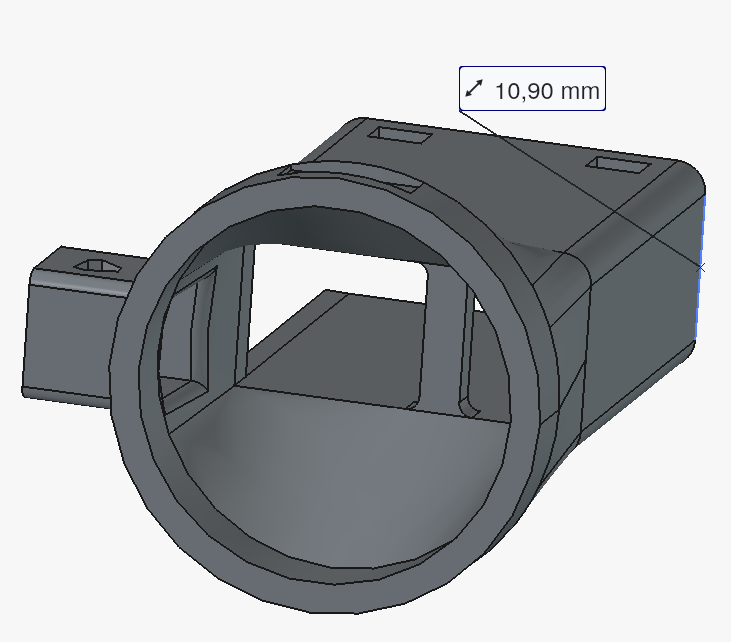
\includegraphics[width=\textwidth]{images/interferometer_holder.png}
        \caption{Interferometer holder}
        \label{fig:interferometer_holder}
    \end{subfigure}\hfill
    \begin{subfigure}{0.45\textwidth}
        \centering
        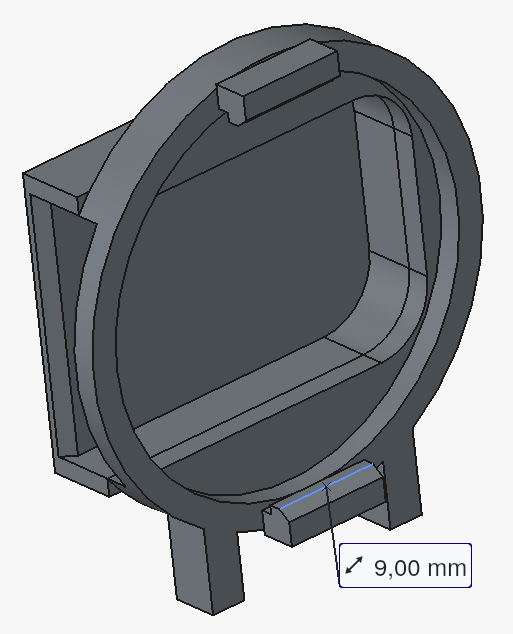
\includegraphics[width=\textwidth]{images/c270_holder.png}
        \caption{Camera sensor holder}
        \label{fig:camera_holder}
    \end{subfigure}
    \caption{3D printed modules. a) Interferometer holder; b) Camera sensor holder, interchangeable and fitted into the coupling.}
    \label{fig:printed_parts_main}
\end{figure}



\subsection{Interferometer holder} The interferometer holder \cref{fig:interferometer_holder} fixes the interferometer casing in a conical seat, and a retaining bar prevents it from sliding out, so the optical unit stays in a repeatable position.

\subsection{Interchangeable camera holder} The camera sensor holder \cref{fig:camera_holder} fits into the coupling \cref{fig:coupling} and can be swapped for other holders, which makes the design modular. It also allows positioning the sensor along the optical path.

\begin{figure}[htbp]
    \centering
    \begin{subfigure}{0.45\textwidth}
        \centering
        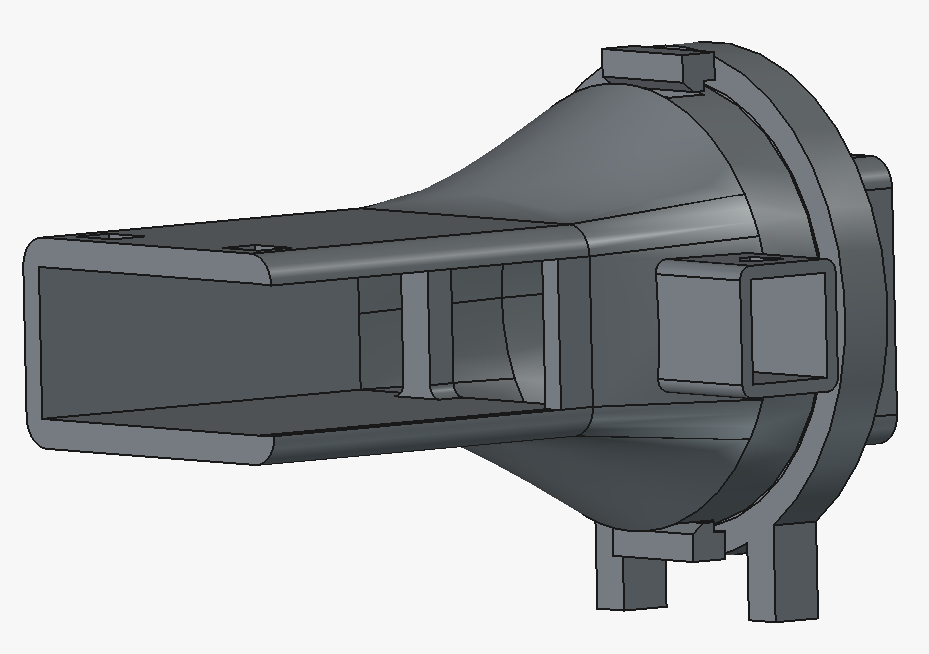
\includegraphics[width=\textwidth]{images/coupling.png}
        \caption{Coupling}
        \label{fig:coupling}
    \end{subfigure}\hfill
    \begin{subfigure}{0.45\textwidth}
        \centering
        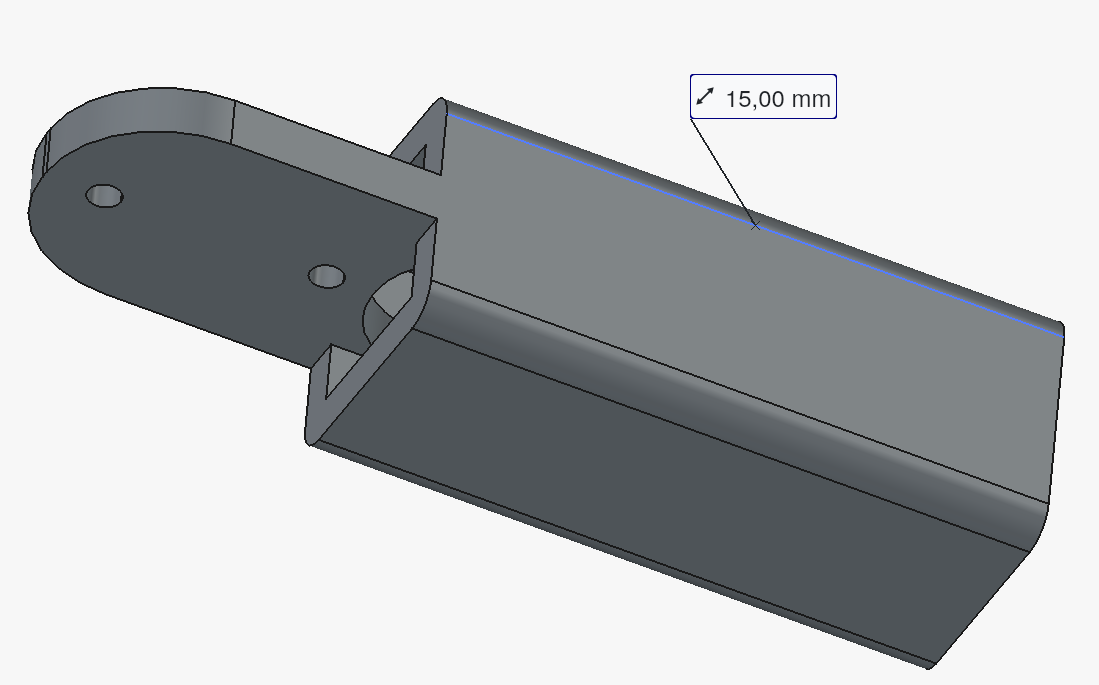
\includegraphics[width=\textwidth]{images/photodiode_holder.png}
        \caption{Photodiode holder}
        \label{fig:photodiode_holder}
    \end{subfigure}
    \caption{3D printed modules. a) Coupling between the interferometer holder and the camera sensor holder, with a square opening for the photodiode holder; b) Photodiode holder, inserted through the square opening of the coupling.}
    \label{fig:printed_parts_detectors}
\end{figure}

\subsection{Coupling} The coupling \cref{fig:coupling} attaches to the interferometer holder and extends the optical path to the detectors with a closed channel that also shields the sensors from ambient light. It houses the camera sensor holder \cref{fig:camera_holder} and has a square opening through which the photodiode holder is introduced.



\subsection{Simultaneous use of photodiode and camera} The photodiode holder \cref{fig:photodiode_holder} slides in through the square opening of the coupling, so it can be placed or removed without dismounting the camera module. This allows using both detectors at the same time and taking advantage of each one (see \cref{sec:c270} and \cref{sec:circuit_schematic}):

\begin{itemize}
    \item \textbf{Photodiode:} its high sampling rate counts the fringes continuously, so no counts are lost even at velocities where the camera, limited to $30\text{ fps}$, would miss fringes.
    \item \textbf{Camera:} it provides the direction of the fringe movement (\cref{sec:roi_fringe_velocity}), and its spatial information can be used to interpolate between fringes and reach a higher spatial resolution than the half-wavelength step of simple fringe counting.
\end{itemize}

\begin{figure}[htbp]
    \centering
    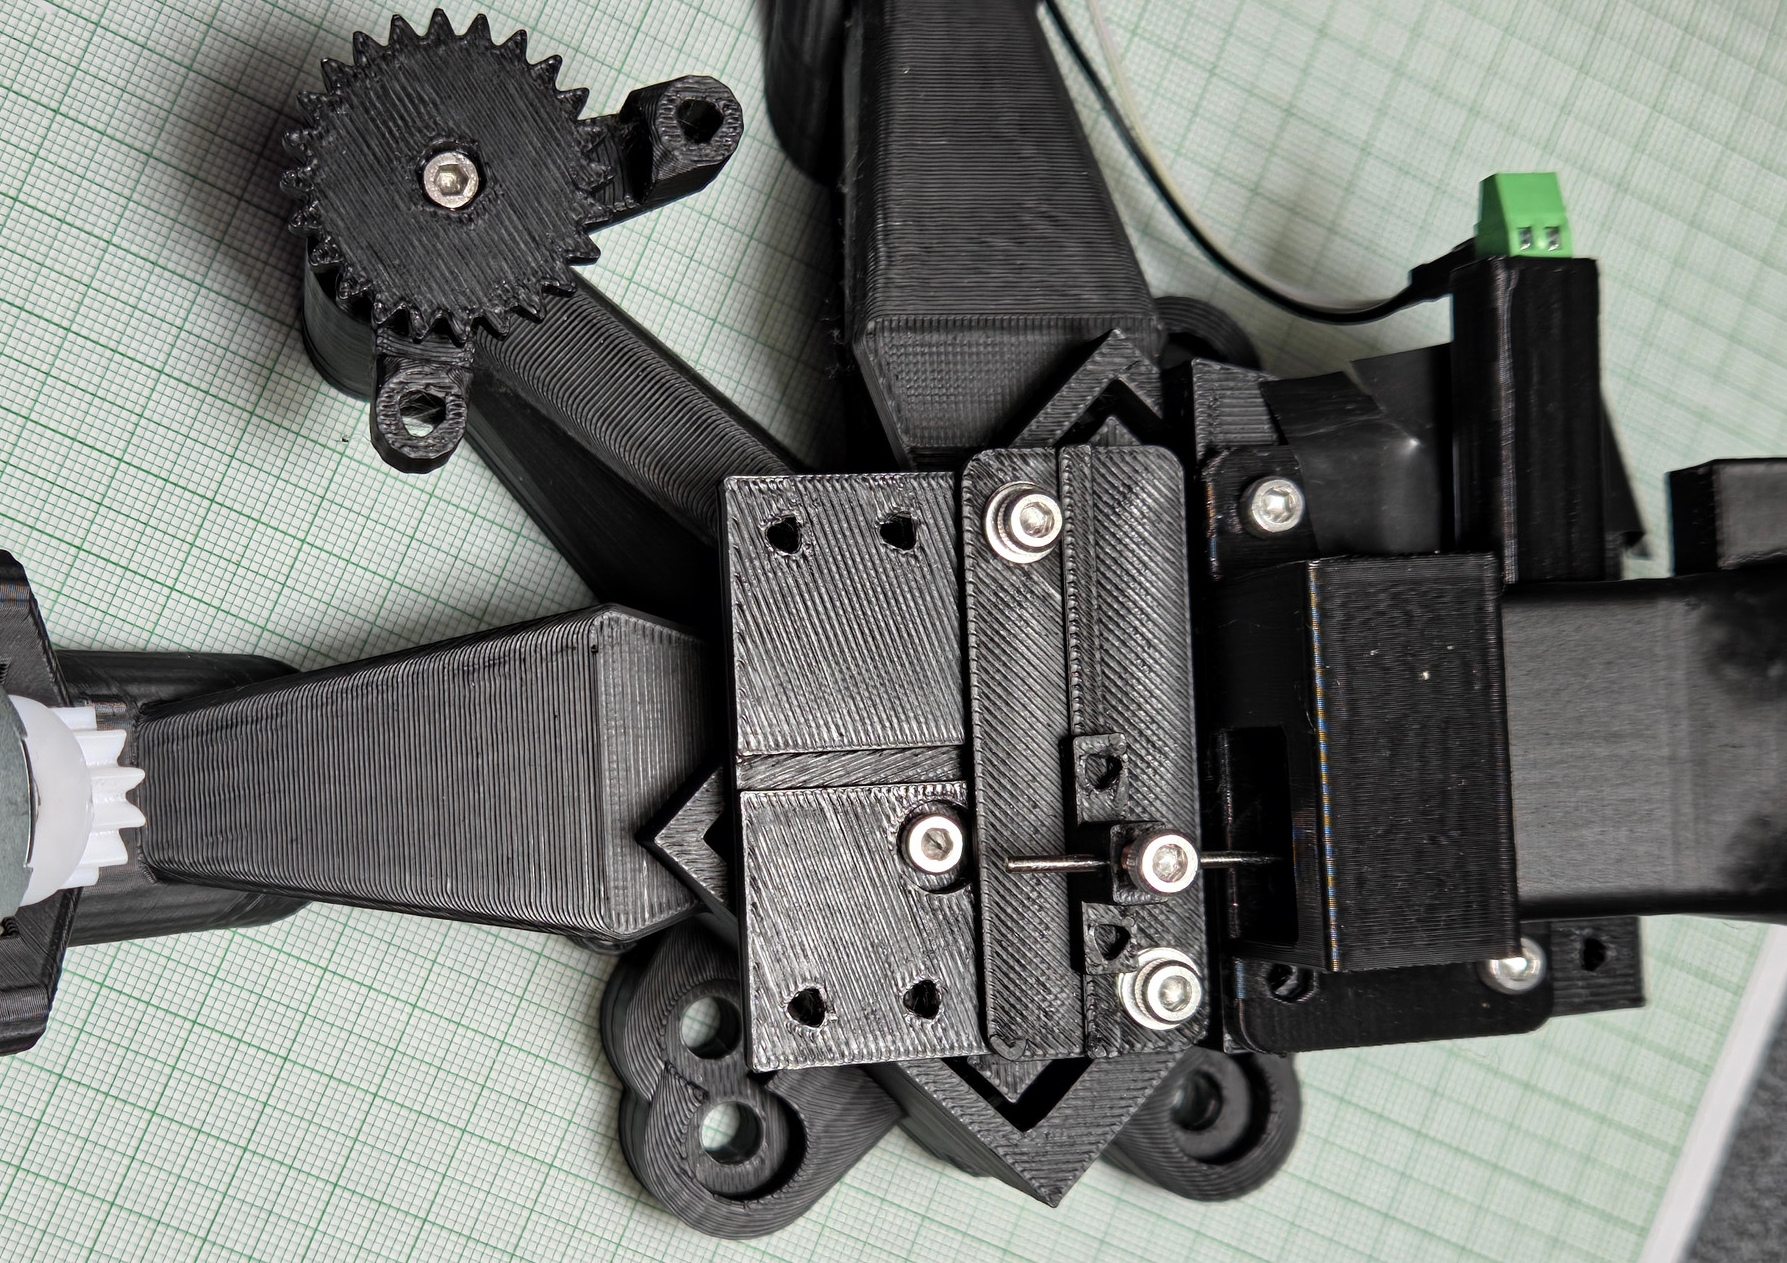
\includegraphics[width=0.55\textwidth]{images/openflexure_with_mountings_compressed_2.jpg}
    \caption{Top view of the final assembly: interferometer, coupling and detector modules mounted on the OpenFlexure Block stage \cite{mengOpenFlexureBlockStage2020}.}
    \label{fig:openflexure_top_view}
\end{figure}

\cref{fig:openflexure_top_view} shows the final assembly used for the calibration. The interferometer holder, the coupling and the detector modules are mounted directly on the OpenFlexure Block stage, forming a single compact block.

An important result of this design is that the system works without an optical table or any vibration-damping platform. Because all the optical components are small and rigidly joined in one compact body, external vibrations move the whole assembly almost equally, so the relative motion between the beam splitter, the mirrors, the lens and the detectors stays very low. Since the fringe pattern depends only on this relative displacement, the measurement is largely insensitive to ambient vibration, which reduces cost and makes the system easy to use outside of a specialized optics laboratory.




\section{Openflexure Calibration Results and Kinematic Analysis}
\label{sec:calibration_results}

To characterize the displacement of the 3D-printed OpenFlexure Block Stage \cite{mengOpenFlexureBlockStage2020}, bidirectional calibration sweeps were performed across five-step counts ($N \in \{1000, 1500, \\ 2000, 2500, 3000\}$) in both positive and negative directions, each sweep for step size was measured 5 times, at a commanded cruise speed of $55\text{ steps/s}$ and acceleration of $150\text{ steps/s}^2$, recorded at $29.0\text{ fps}$ (\cref{fig:openflexure_cal,fig:single_run_1000}).

\begin{figure}
    \begin{center}
        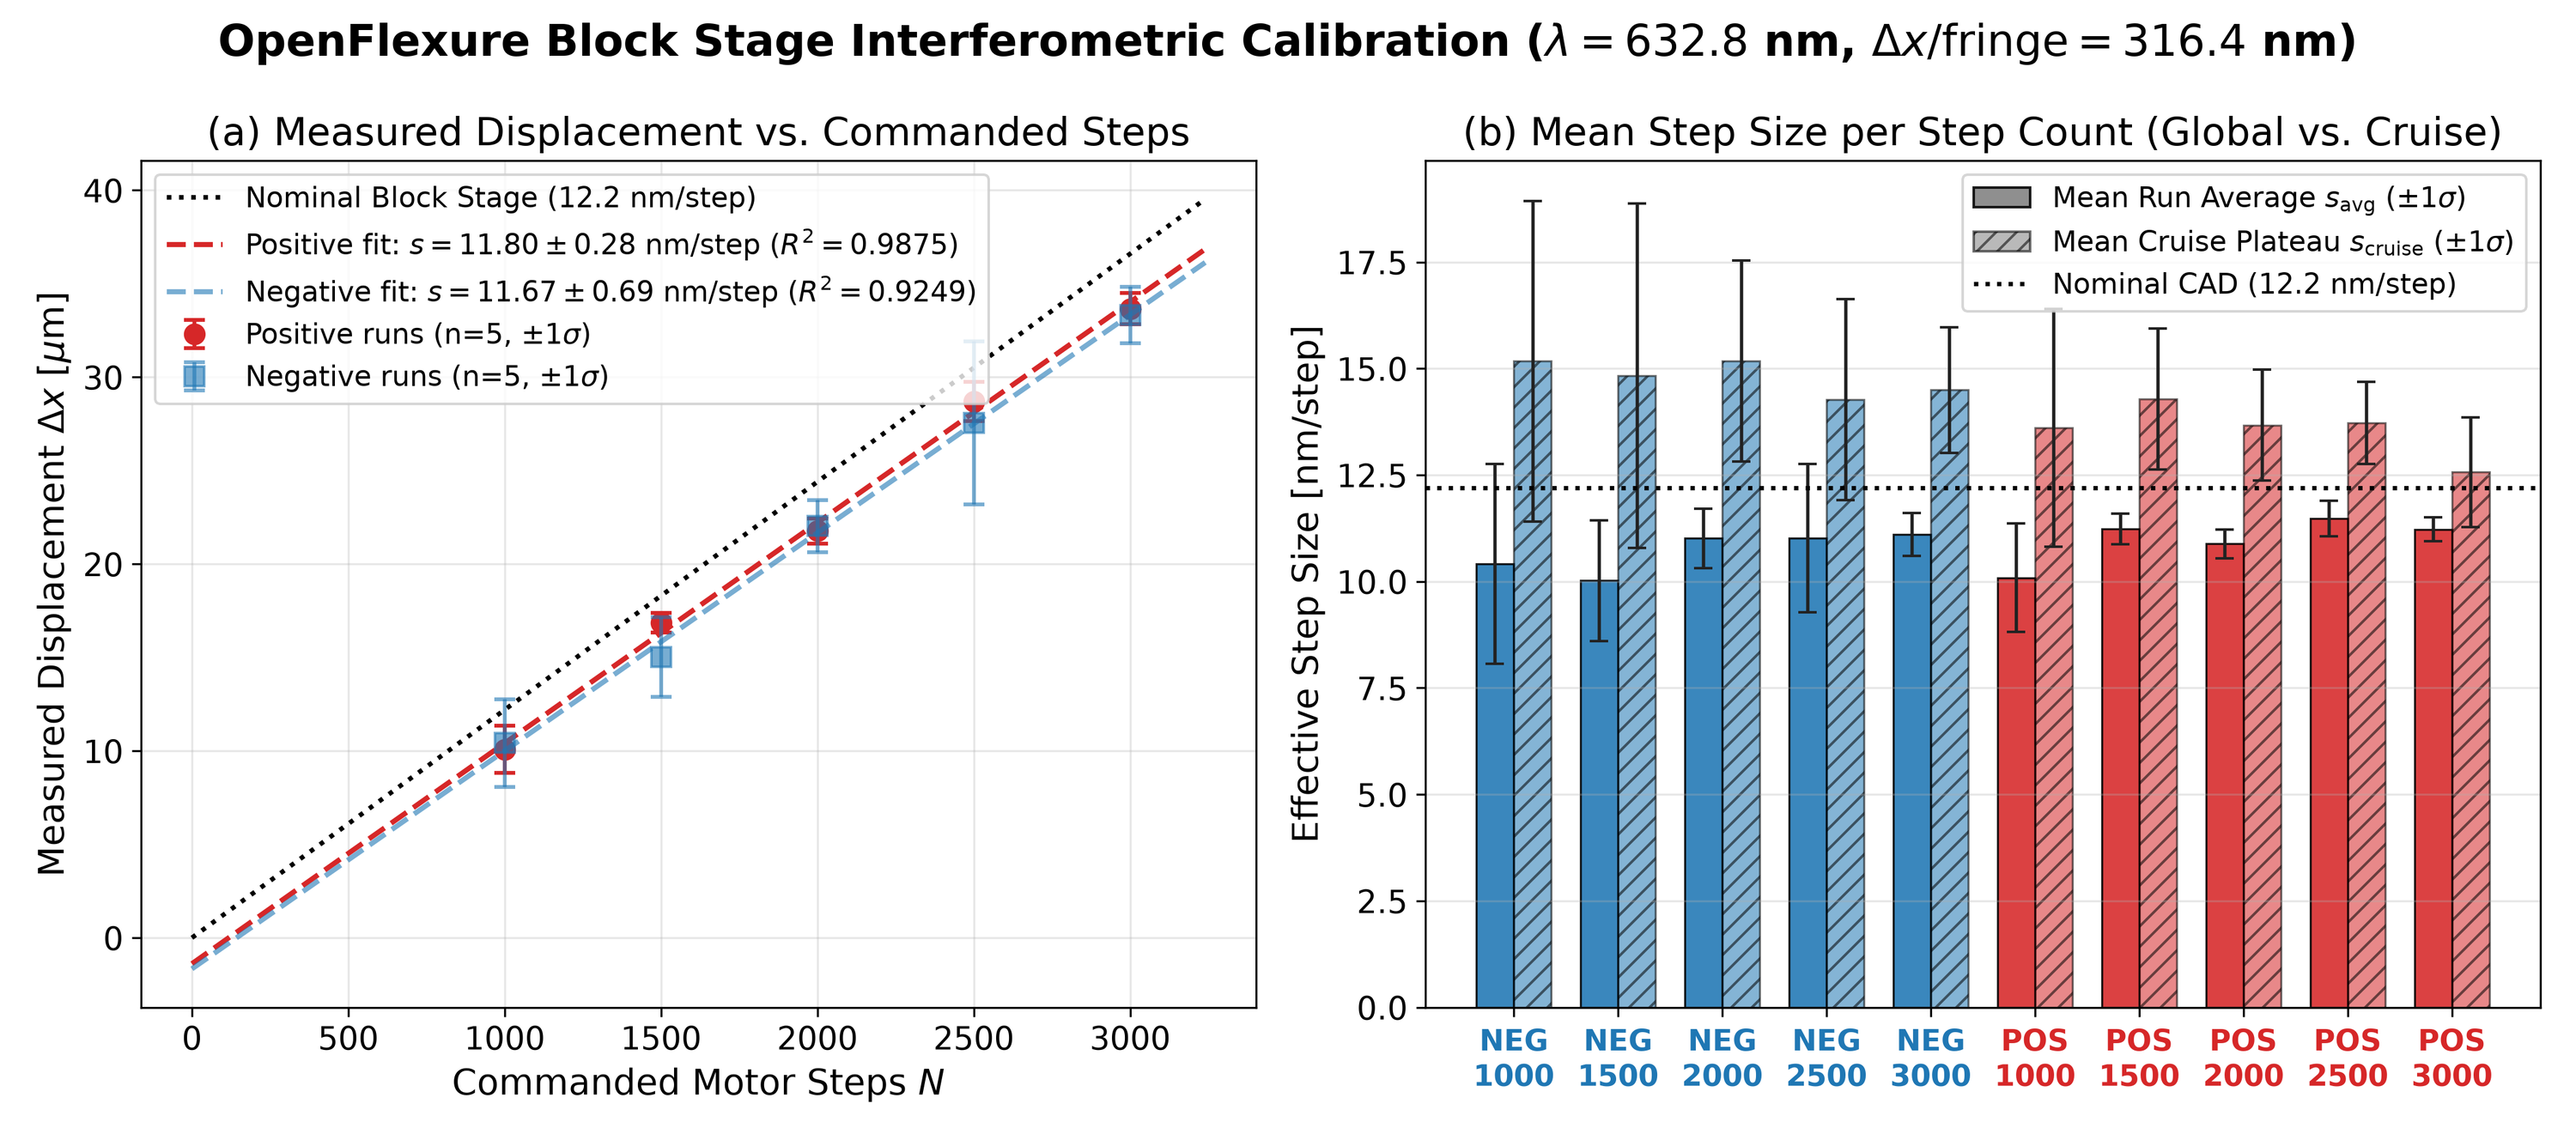
\includegraphics[width=15cm]{images/openflexure_calibration.png}
    \end{center}
    \caption{Openflexure calibration of step size. Blue: negative direction; red: positive direction.}
    \label{fig:openflexure_cal}
\end{figure}

\subsection{Definition of Plot Metrics}
\label{sec:plot_metrics}
\begin{itemize}
    \item \textbf{Nominal CAD ($12.2\text{ nm/step}$):} Here, \textbf{CAD} stands for \textit{Computer-Aided Design}. This dotted reference line represents the idealized theoretical step size derived from the Block Stage geometric design assuming zero backlash, rigid plastic links, exact M3 lead-screw pitch ($0.5\text{ mm/rev}$), $2:1$ external gear reduction, $4096$ half-steps/rev on the 28BYJ-48 motor, and the $5:1$ flexure lever reduction ($\approx 12.2\text{ nm/step}$) \cite{mengOpenFlexureBlockStage2020}.
    \item \textbf{Run Average ($s_{\text{avg}}$):} The global effective step size over an entire sweep, computed as $s_{\text{avg}} = \Delta x_{\text{total}} / N$, where $\Delta x_{\text{total}} = m\,\frac{\lambda}{2}$ ($316.4\text{ nm/fringe}$ at $\lambda = 632.8\text{ nm}$). Because $s_{\text{avg}}$ divides total displacement by total commanded steps, it includes any startup deadband, stiction, and deceleration losses.
    \item \textbf{Instantaneous Step Size:} Computed from the frame interval $\Delta f$ between consecutive peaks (or troughs) as $s_{\text{inst}} = \frac{(\text{FPS}/\Delta f)\,(\lambda/2)}{v_{\text{cmd}}}$, showing how the effective mechanical sensitivity evolves over the duration of a single sweep.
    \item \textbf{Cruise Plateau ($s_{\text{cruise}}$):} The median of the upper $40\%$ fastest fringe intervals during a sweep, isolating the steady-state motion regime once the motor has overcome initial static friction and gearbox take-up.
\end{itemize}



\subsection{Single-Run Dynamic Behavior}

\begin{figure}
    \begin{center}
        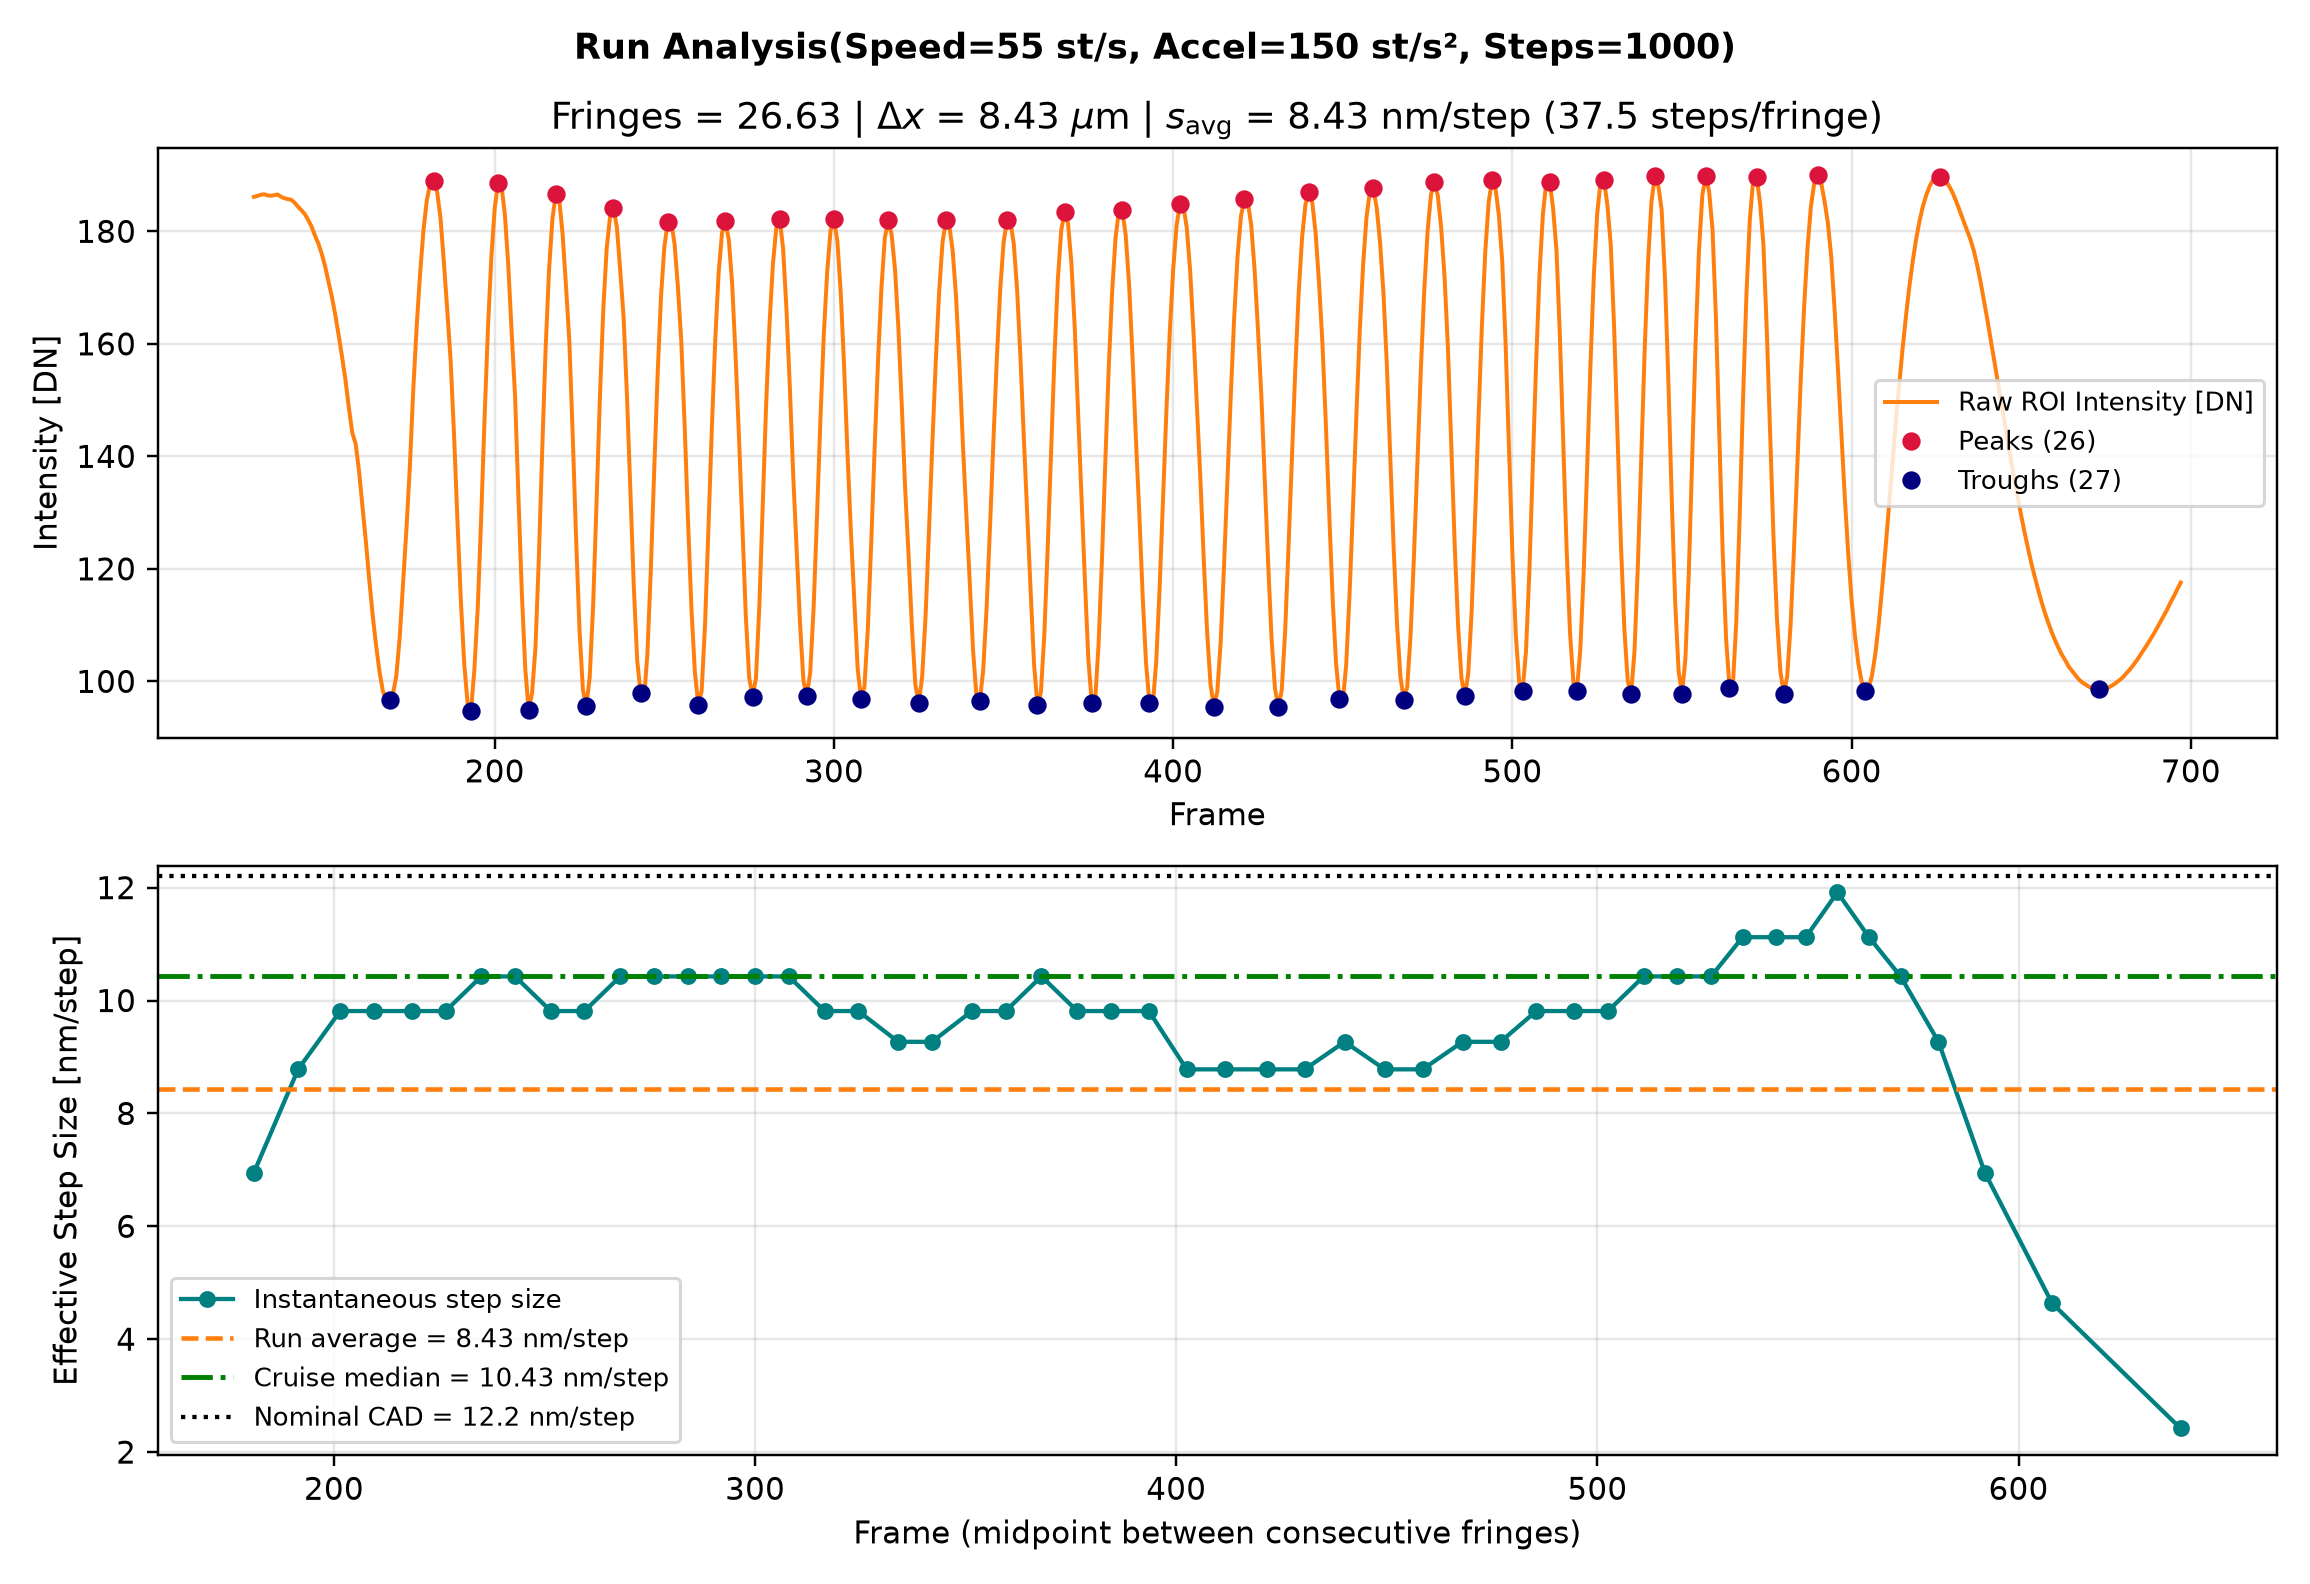
\includegraphics[width=14cm]{images/55_150_positive_1000_analysis.png}
    \end{center}
    \caption{Openflexure calibration of step size (1000 steps single run).}
    \label{fig:single_run_1000}
\end{figure}

\cref{fig:single_run_1000} illustrates a complete $1000$-step positive sweep after preloading. Across the trimmed active window, the algorithm detects $26$ peaks and $27$ troughs, yielding $26.63$ fringes ($\Delta x = 8.43\ \mu\text{m}$) and a global run average of $s_{\text{avg}} = 8.43\text{ nm/step}$ ($37.5\text{ steps/fringe}$). Three distinct physical phases appear in the instantaneous step-size curve (bottom panel):
\begin{enumerate}
    \item \textbf{Breakaway and Ramp-Up (Frames $180\text{--}210$):} The effective step size starts near $7.0\text{ nm/step}$ and rises rapidly as the motor accelerates ($55/150 \approx 0.37\text{ s}$) and overcomes initial static friction in the gear train and M3 nut.
    \item \textbf{Steady-State Cruise Plateau (Frames $210\text{--}570$):} The stage settles into uniform periodic motion around a cruise median of $s_{\text{cruise}} = 10.43\text{ nm/step}$ (hovering between $8.8$ and $11.9\text{ nm/step}$).
    \item \textbf{Deceleration and Relaxation (Frames $575\text{--}675$):} Once the motor finishes its $1000$ steps and de-energizes its coils, the fringe period widens smoothly and $s_{\text{inst}}$ tapers down toward $2.4\text{ nm/step}$ as the 3D-printed PLA flexure relaxes mechanically. This transient startup/stopping overhead explains why $s_{\text{avg}} = 8.43\text{ nm/step}$ lies below $s_{\text{cruise}} = 10.43\text{ nm/step}$.
\end{enumerate}

\subsection{Linear Regression and Bidirectional Symmetry}
\cref{fig:openflexure_cal}(a) plots total measured displacement $\Delta x$ against commanded steps $N \in \{1000, 1500, 2000, 2500, 3000\}$, with $n = 5$ repeated trials per step count in each direction ($25$ runs per direction, error bars indicating $\pm 1\sigma$ trial-to-trial standard deviation). Linear least-squares fits across all runs reveal strong linearity in both actuation directions:
\begin{align}
    \text{Positive direction:}\quad s_+ &= 11.80 \pm 0.28\text{ nm/step} \quad (R^2 = 0.9875) \\
    \text{Negative direction:}\quad s_- &= 11.67 \pm 0.69\text{ nm/step} \quad (R^2 = 0.9249)
\end{align}
Both calibrated incremental slopes agree closely with the $12.2\text{ nm/step}$ nominal CAD value within experimental uncertainty (differing by only $3.3\%\text{--}4.3\%$) and agree with each other within $\sim 1.1\%$, confirming consistent bidirectional sensitivity once preloaded. The negative direction exhibits slightly larger run-to-run dispersion ($\pm 0.69\text{ nm/step}$ and wider $\pm 1\sigma$ error bars at $N = 1500$ and $2500$) than the positive direction ($\pm 0.28\text{ nm/step}$), reflecting minor mechanical asymmetry between pushing against and relaxing with the PLA flexure restoring force and gear mesh. Crucially, both regressions share a small negative $y$-intercept ($\approx -1.4\text{ to }-1.5\ \mu\text{m}$), capturing a nearly constant startup loss prior to rigid engagement. Because this startup offset is absorbed into the intercept rather than the slope, multi-step linear regression accurately recovers the true incremental stage sensitivity ($\sim 11.7\text{--}11.8\text{ nm/step}$) even when single-run averages are pulled down at shorter travels ($N = 1000$).

Finally, \cref{fig:openflexure_cal}(b) compares the grouped mean values ($\pm 1\sigma$, $n = 5$) of $s_{\text{avg}}$ and $s_{\text{cruise}}$ across each step count and direction. As expected, $s_{\text{avg}}$ climbs steadily toward $\sim 11\text{--}11.5\text{ nm/step}$ for larger step counts ($1500\text{--}3000$ steps) as the initial compliance transient becomes proportionally smaller relative to total travel. Meanwhile, the $s_{\text{cruise}}$ averages consistently sit slightly above the $12.2\text{ nm/step}$ nominal line ($\sim 13\text{--}16\text{ nm/step}$, with individual runs peaking near $\sim 20.8\text{ nm/step}$); this occurs because taking the upper $40\%$ fastest intervals biases toward integer-frame rounding at smaller $\Delta f$ ($29.0\text{ fps}$) and captures brief elastic spring-forward bursts immediately following static friction breakaway, alongside minor tooth-to-tooth variability in the printed gear mesh.

\subsection{Mirror Velocity from the Fringe Rate}
\label{sec:openflexure_velocity}

The same fringe traces give the velocity at which the stage was moving. Applying \cref{eq:velocity_fringe_rate} to every interval between consecutive peaks (or troughs), the fringe-crossing frequency is $f_{\text{fringe}} = f_s/\Delta f$, with $f_s = 29.0\text{ fps}$ and $\Delta f$ the number of frames of the interval, and the mirror speed is $v_{M2} = \frac{\lambda}{2}f_{\text{fringe}}$, with $\lambda/2 = 316.4\text{ nm}$. The sign of the velocity is taken from the commanded direction, since a single ROI trace cannot resolve it (\cref{sec:roi_fringe_velocity}). The mean velocity of a run is its displacement divided by the duration of the active window, and the cruise velocity is the median over the $40\%$ fastest intervals, as for $s_{\text{cruise}}$. The expected (theoretical) velocity is the commanded speed multiplied by the displacement per step of the stage, $v_{\text{expected}} = v_{\text{cmd}}\,s$. With the nominal CAD step $s = 12.2\text{ nm/step}$, obtained from the geometry of the Block Stage (\cref{sec:plot_metrics}), the commanded $55\text{ steps/s}$ give $v_{\text{expected}} = 55 \times 12.2\text{ nm} = 0.671\ \mu\text{m/s}$, which corresponds to a fringe rate of $2.1\text{ Hz}$. Using the calibrated slopes of the regression instead, $s_+ = 11.80\text{ nm/step}$ and $s_- = 11.67\text{ nm/step}$, gives $0.649\ \mu\text{m/s}$ and $0.642\ \mu\text{m/s}$.

\begin{figure}[htbp]
    \centering
    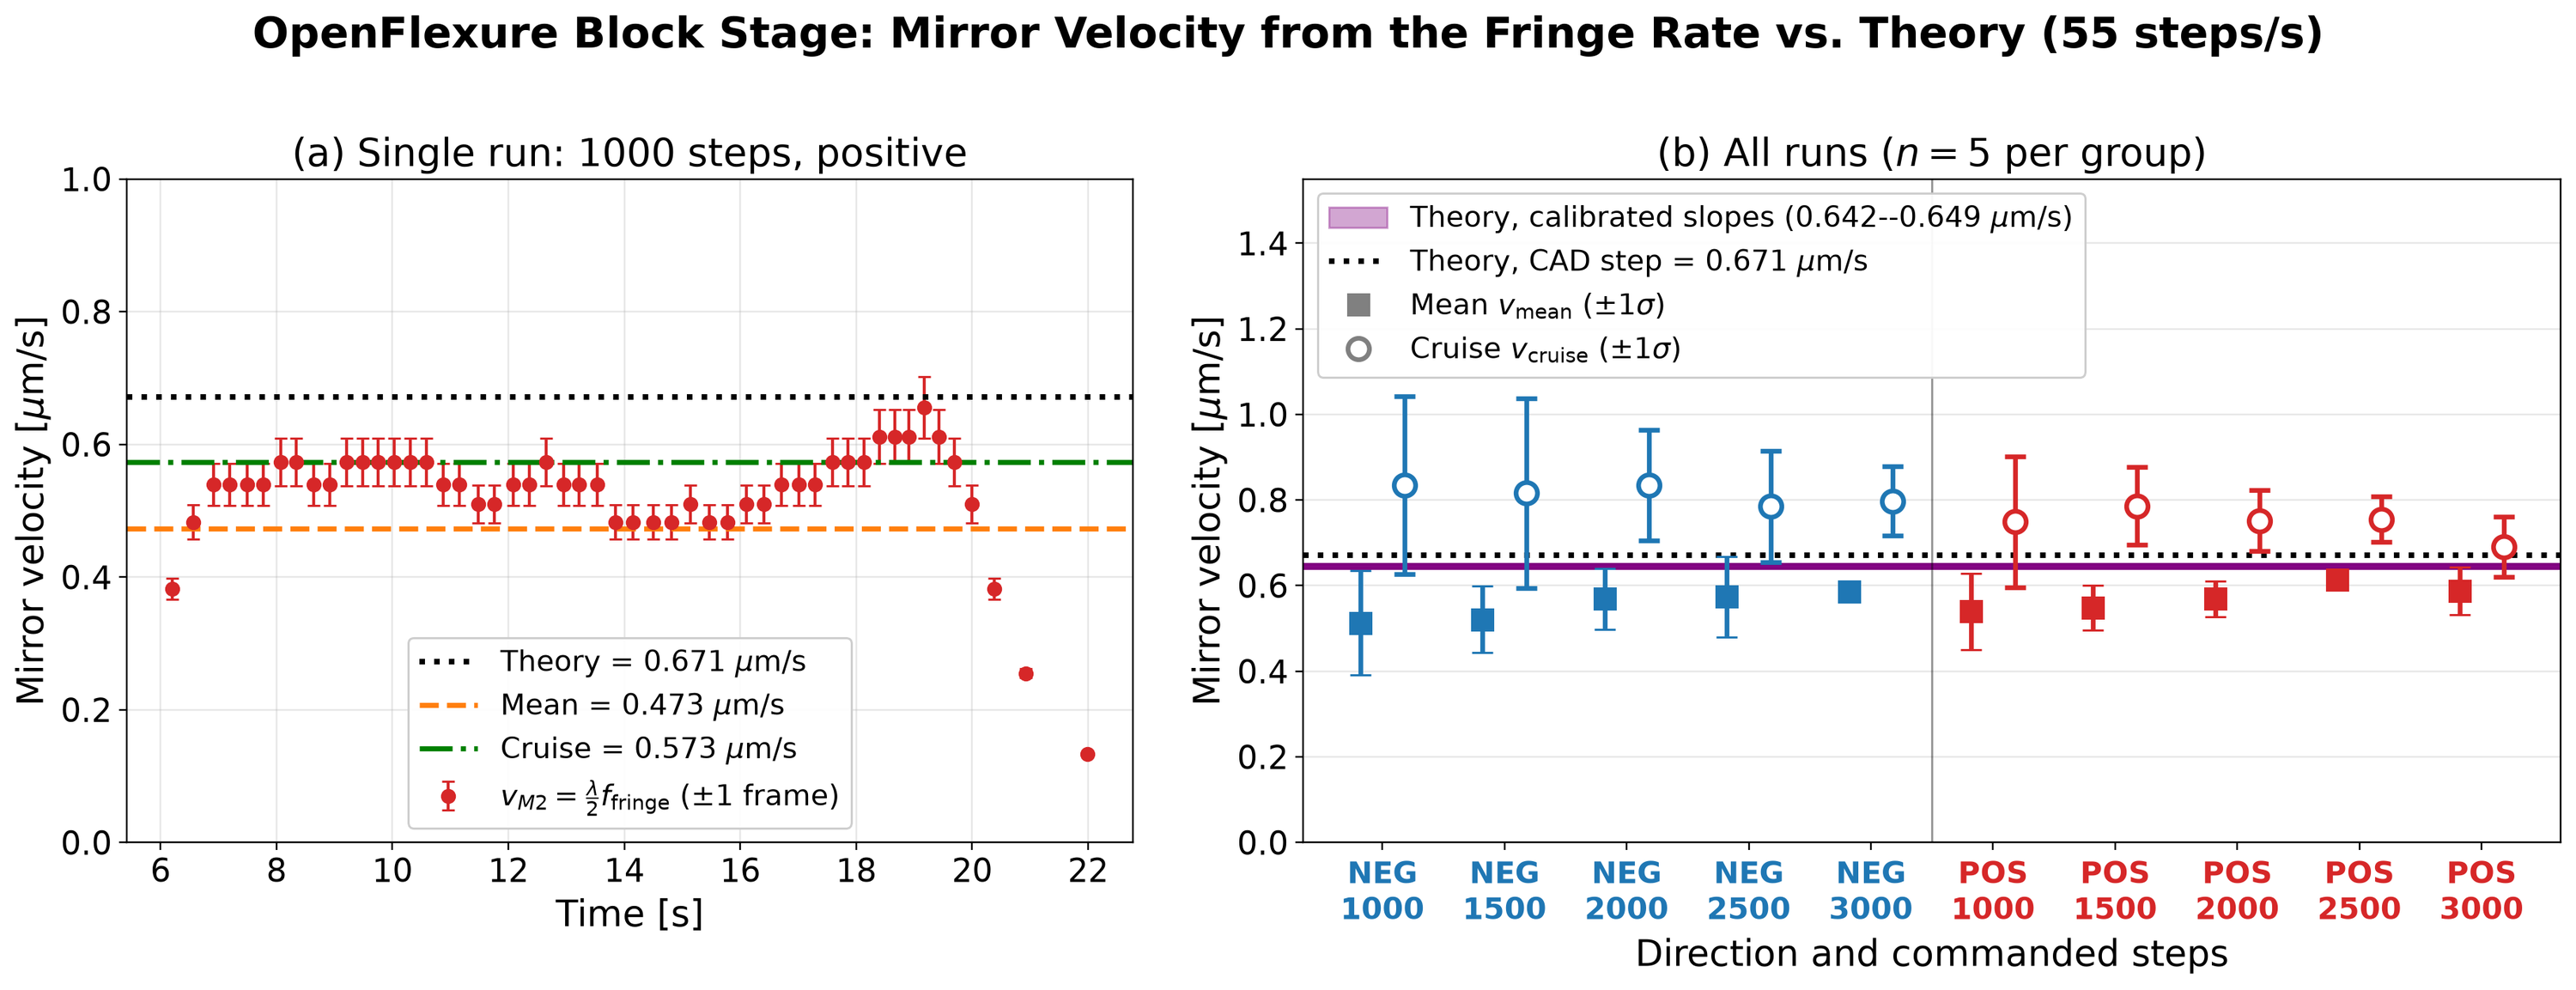
\includegraphics[width=\textwidth]{images/openflexure_velocity.png}
    \caption{Mirror velocity obtained from the fringe rate with \cref{eq:velocity_fringe_rate} compared with the theoretical velocity. a) Velocity of each fringe interval of the $1000$-step positive sweep of \cref{fig:single_run_1000}, with the error bars of $\pm 1$ frame of the interval, the run mean, the cruise median and the theoretical value of $0.671\ \mu\text{m/s}$; b) mean (squares) and cruise (circles) velocities ($\pm 1\sigma$, $n = 5$) of every direction and step count against the theoretical value, and the band (purple) of the values obtained with the calibrated slopes. Blue: negative direction; red: positive direction.}
    \label{fig:velocity_1000}
\end{figure}

\cref{fig:velocity_1000}a shows the velocity of the $1000$-step sweep. The velocity rises from about $0.4\ \mu\text{m/s}$ during the acceleration ramp, stays around a cruise value of $0.57\ \mu\text{m/s}$ and drops during the deceleration, following the three phases described for the instantaneous step size. The error bars are the uncertainty of one frame in the length of each interval, $\delta v = v/\Delta f$, about $6\%$ in the plateau. The cruise value is below the theoretical $0.671\ \mu\text{m/s}$, which corresponds to the cruise step of $10.43\text{ nm/step}$ of this run, and the mean is lower still because it includes the ramps. \Cref{fig:velocity_1000}b compares all the sweeps with the theoretical velocity: the mean velocities lie below it and the cruise velocities above it, and the band obtained with the calibrated slopes falls between both.

\begin{table}[htbp]
\centering
\caption{Mirror velocity measured from the fringe rate in the $50$ calibration sweeps ($55\text{ steps/s}$, $150\text{ steps/s}^2$, mean $\pm 1\sigma$ over runs), compared with the expected velocity obtained with the CAD step ($12.2\text{ nm/step}$) and with the calibrated slope of each direction.}
\label{tab:openflexure_velocity}
\begin{tabular}{lccccc}
\hline
Direction & Runs & $v_{\text{mean}}$ [$\mu$m/s] & $v_{\text{cruise}}$ [$\mu$m/s] & $v_{\text{CAD}}$ [$\mu$m/s] & $v_{\text{cal.}}$ [$\mu$m/s] \\
\hline
Positive & $25$ & $0.571 \pm 0.058$ & $0.746 \pm 0.092$ & $0.671$ & $0.649$ \\
Negative & $25$ & $0.553 \pm 0.083$ & $0.813 \pm 0.150$ & $0.671$ & $0.642$ \\
All      & $50$ & $0.562 \pm 0.071$ & $0.780 \pm 0.128$ & $0.671$ & $0.642$--$0.649$ \\
\hline
\end{tabular}
\end{table}

\Cref{tab:openflexure_velocity} summarizes the velocity of all sweeps, together with the expected velocity of each direction computed with its calibrated slope. The mean velocity, $0.562 \pm 0.071\ \mu\text{m/s}$, is lower than the expected one because it includes the acceleration ramp, the breakaway and the relaxation at the end of each sweep; consistently, it grows with the number of steps, from $0.526 \pm 0.102\ \mu\text{m/s}$ for $N = 1000$ to $0.586 \pm 0.041\ \mu\text{m/s}$ for $N = 3000$, as these transients weigh less. The cruise velocity, $0.780 \pm 0.128\ \mu\text{m/s}$, is above the expected value, which is the same bias already discussed for $s_{\text{cruise}}$: it selects the fastest intervals, and at $29\text{ fps}$ an error of one frame in an interval of about $16$ frames changes the velocity by $\sim 6\%$. The expected value computed with the calibrated slopes, $s_+ = 11.80\text{ nm/step}$ and $s_- = 11.67\text{ nm/step}$, is $0.649\ \mu\text{m/s}$ and $0.642\ \mu\text{m/s}$, between the mean and the cruise values. The negative direction shows the larger dispersion, in agreement with the mechanical asymmetry found in the regression. Finally, the fastest intervals correspond to fringe rates below about $4.5\text{ Hz}$, so even then there are more than $6$ frames per fringe and the velocities are far from the aliasing limit of the camera (\cref{sec:camera_velocity}).
